\setcounter{chapter}{ 2 }
\chapter{\textbf{Cardoza Station, Part 1} }



\subChapterTitle{``Drowning in Pudding''} 

\deets{Ion}{July 12, 2012}



\jumpHeadline{ Shore Leave! } 


\sceneHeadline{Shore Leave: Jaya }

Padme (Jaya's sister)'s son Simon has been sent to the mines.  Padme doesn't seem too concerned but Jaya wants to get him back.  Padme has recently given birth to Micah, and tattoos with the kid on her lap.  Both sisters are openly disappointed that it's another son.  Banter ensues, with the sisters cheerfully insulting each other, Jaya telling Padme ``you are great at tattooing but not good with kids'', and Padme asking Jaya why she doesn't have kids yet.  Jaya wants to get Simon back but Padme doesn't see the point in spending money on him.  Jaya seems to care about having ``a good kid'' not be wasted, but Padme believes she's just doing this to avoid having children of her own.  Jaya denies it vehemently ... so it must be true.


\sceneHeadline{Shore Leave: Hayley }

Hayley is in the gym.  She was gone from her ``main contract'' for several days on the last mission.  Her employer is disgruntled about her absence.  Hayley points out that she can't just leave.  She's at the bottom of the social structure, which she believes is very strange.  She doesn't understand the military ranks, and believes that they violate the natural order (by Citizens being lower rank than Nationals for instance).  ``Power seems to be expressed by belittling other people''.  This her employer feels is at least right and proper: ``Some people should be put in their place''.  Now we get to the meat of things: her employer wants to know exactly what Hayley's patrol squad has been doing.  Hayley explains about the new station and the mission to find (Trenton) and re-open the station.  She gives her a crudely drawn map of the area around New Station that you could see from Trenton's building's rooftop.  Her employer finds this somewhat comprehensible.  Hayley tries to ask about the codes that control the trains but her employer doesn't find it believable that trains are controlled by codes.  Hayley did write what numbers she could see from seeing Trenton's book, but they are not complete or comprehensible, being mostly just random numbers and squiggles since she doesn't know mathematical symbols or formulae. Gillian believes she can find someone who knows how to interpret them {[}Suko's note: But it will be next to useless since they are the equivalent of seeing half of a page of a 100 page mathematical expression, while looking at it upside down{]}.  Hayley says there is more information in her reports that were submitted, presumably separately.  Her employer is somewhat insistent that Hayley come back soon.  DeVries (a Citizen that she dislikes) is becoming a real problem for her.  Hayley doesn't see an easy way to get sent back from the TA other than getting severely injured... which she expresses a preference for avoiding since it counters her contract holder's instructions to avoid getting killed.  They agree to have her uniform re-fitted by the house seamstress (!).


\sceneHeadline{Shore Leave: Oliver }

Oliver is in his room trying to get undressed and wind down.  His mother comes in to tell him something, but sees his war wound and gets suddenly withdrawn (embarrassed?  unclear).  They make awkward small talk.  He complains about the rest of his team, how they are incompetent and don't know what they are doing.  He's not happy that he is reporting to a Franchise person.  She wants him to meet with people who can further his career and get out of his niche.  Mostly it's uncomfortably oblique, until Oliver directly asks if she can put him in touch with someone.  Ironically she wanted to do just that, but they are interrupted by the dinner bell, and the conversation goes unsaid.


\sceneHeadline{Shore Leave: Jonah }

Jonah is working with his cover identity.  He is being asked by his bandage supplier (one of his reliable suppliers) to get some application forms for the medic academy for the supplier's son (Mika).  Jonah promises to look into getting the form.  He is pretty sure he can't get the form and gets the run around at the academy, but he tries.  He talks up a young man at a desk and finds out that the best way is to get a Citizen to get an appointment with a dean who can get you an application form.  This being infeasible, to put it mildly, Jonah then talks to one of his street medic friends to see if he wants an apprentice.  The friend says he'll consider it and for Jonah to set up some kind of meeting.  Jonah goes back to his bandage supplier and convinces him that getting into the academy is tricky but that his son's odds are improved by having experience, so he should consider getting him apprenticed.



\jumpHeadline{Session } 



Oliver at the medic's.  They get along \textit{fabulously}, the doctor taking blood samples and Oliver giving her a hard time for every procedure.  She asks Oliver about the leg which he tries to avoid talking about but she presses on telling him the missions need everyone to be in good shape.  {[}Out of nowhere an out-of-game cat bolts across the hall, leaving all characters strangely confused{]}.  The doctor prescribes that Oliver go down twice a week to the cistern and swim.  Oliver claims that there are deep bone injuries that can't be fixed by swimming which he's already had a doctor look at.  She calls his bluff saying that that's not his actual problem.  The leg can be fixed eventually but that's not his issue, and does he want her to spell it out?  Oliver quickly retreats without admitting anything saying the exercise will be great.  He calls her ``ma'am'' and winks at her on the way out.


\memoryScene{
Notes:

- The leg can be fixed?

- The doctor is Morgan's sister.
}


Jaya gets called by the intercom and folds at cards.  She's happy, so she gets Oliver's last name totally wrong.  The room she goes to has empty tanks (cisterns?) ... and Morgan.  Jaya saunters in and straightens up abruptly when she sees Morgan.  Morgan tells her she finds Jaya's (or the team's?  It was unclear) performance mediocre.  Jaya tries to claim that the team's performance is basically par.  Morgan says that she was under constraints for choosing who would be on the team, constraints which in this case were apparently mostly medical.   She adds that the team with some work can be adequate.  She says that ``we'' (the Directorate?) have enemies.  Jaya says ``Nicklepan'' but Morgan corrects her saying that Anglia is actually who she is referring to.  She expects that the team can be made better but expects Jaya to rise to the cause.   Jaya is clearly intimidated by the idea but says she can do it and stammers her way out.


\memoryScene{
Notes:

- The constraints for team selection were medical.  (Medical???)
}


Trenton comes to the barracks.  Hayley opens the door.  When Jaya says ``close the door'' Hayley shuts it in his face.  Trenton comments on Hayley's literalness (and pliability?).  He invites Jonah to follow him.  They walk out to a door that says ``machine shop'' saying he needs a ``pair of steady hands''.  Jonah notes that he is pleased they let him walk around, and inquires as to where Trenton actually is most of the time, to which Trenton replies obliquely: ``around''.  They banter about Morgan's sex life (scary!) then Trenton tells Jonah that they are hooking radios to the trains.  Trenton shows him how they work, and Jonah is (unusually) visibly impressed.  Trenton explains a little bit about them.  Trenton then asks Jonah if he knows where they are.  Jonah replies that he tries not to ask questions he won't get answers to.  Trenton continues on conspiratorially that he thinks even the DIrectorate doesn't know where they all are because Morgan doesn't want them to know.  He asks if Jonah has considered that SAC-9 means there are at least 8 other SACs.  Jonah says he doesn't even know what a SAC is.  After Trenton explains he says these are places the TA must've rediscovered recently, but how long ago? Trenton then points out a noise on the wall that he can't identify.  Where IS the SAC?  As they part Jonah comments that he's pleased Trenton isn't locked up some place.  Trenton grins and says it's not \textit{him} who's locked up with \textit{them}.



(While he's gone Jaya and Oliver try to explain Hayley that Trenton is trying to get into her pants.  They try to teach her how to say ``No''.  The operation cannot be called a success.)


\memoryScene{
Notes:

- The radios are from Cydonia.

- ``SAC'' means ``Stand-Alone Complex.''
}


Hayley gets summoned somewhere by the guards.   She follows them down the hall, which is  followed by an hour(?) she has no memory of.  When she wakes up she's drowning in a container of purplish-bluish liquid sealed up. There's no breathable air and after a concerted effort to right herself and find a breathable point Hayley starts to panic.  She starts to punch the top to try and get out.  She breaks her hand, sees a dark red in the liquid, blond hair swirling around her head and then passes out.



Hayley wakes up in a bed, a medic? standing over her with a badge that says ``Swan''.  She asks if she had a nightmare and he says no but she did very well.  It was a test, and, when she asks, he has authorization from Dr. Gerhauser who was pleased with the result.



Hayley seems very confused about who Dr. Gerhauser is asking for authorization if it's her contract holder or ``the Agent'' (meaning Morgan).  The medic doesn't really answer the question but tries to make sure Hayley is ok before he sends her back.  Hayley asks if she is the only one who has to undergo the tests and the agent replies that so far yes, but the others will be doing them too.



Hayley is gone for 8 hours.  She comes back in the night.  Oliver wakes up and asks her where she is.  (Jonah listens in without saying anything or showing he's awake.)  She tells him, and when she gets to the part about almost dying, he gets angry and wakes up Jaya and all three interrogate Hayley about what happened.  (Jaya jumps out of bed and salutes, sleepily demanding that everyone be presentable.)  No one is ok with the prospect of being drowned as part of testing.  Jaya and Oliver quarrel about whether they should go back to sleep.  Eventually Oliver says he is going ``swimming'' which makes Jaya and Jonah snort and say ``good one''.  When Oliver leaves with his swim trunks and towel Hayley asks if she can go, and the others stop her assuming Oliver is just jerking her around and wanting some private time.  (The idea of swimming as a non-Citizen isn't just decadent but actively insane, since pools of water are so dangerous.)


\memoryScene{
Notes:

- Agent Morgan Gerhauser's sister is the doctor.
}


Oliver goes down to the cistern to swim.  It's reasonably well lit and deep.  It is \textit{cold} but very relaxing and comforting.  He finds it's pleasant to have the pressure off the leg.   After 15-20 minutes he gets too cold and gets out.  He then goes to practice shooting (though there isn't really a range).  Just as he is coming back the alarms go off.



The red alarms flash, the klaxons shout.  Everyone gets ready to leave.  Oliver shows up as the others are leaving.  There is some confusion as Oliver and Jonah go back to get Oliver's equipment despite Jaya insisting they go as fast as possible.  When they show up at the line-up Morgan isn't obviously more displeased than usual.  She walks towards the train saying she'll brief the squad on the way.  She asks if they are familiar with the name DeVries, noting that they won't have the pleasure of meeting him since he's dead.  {[}Note: Hayley's employer mentioned DeVries being a problem in session 2....{]}  The TA came into the possession of a letter written by DeVries that indicates a rogue Citizen has an explosive device.  The mission is to pursue the man to Cardoza and get back the device and apprehend him before he ... blows up Anglia.   (Jaya gets a clarification about whether the man needs to be alive after apprehensions.)  Then she grits her teeth at Jaya and says ``Impress me'' as she did before.  As the team boards the train Morgan seems unusually tense, like she's doing something distasteful yet also a little eager.



On the way to Cardoza the train goes faster than anyone has ever experienced.  It then decelerates rapidly inducing nausea and causing most of the team to stumble and or fall.

The address is that of Citizen Cyril Magnin.  Oliver knows Cyril Magnin isn't terribly popular, with a reputation as a troublemaker.  He is pro-Directorate and isolationist, believing the Directorate should not have gone to war with Nicklepan or be allied with Anglia.   He is married ,very wealthy and has stakes in a number of companies.  Despite his reputation he has enough influence that people invite him everywhere.



When the doors open there are people waiting with bags looking put out that the train was so abrupt.  There is an altercation between a man who complains about schedules and Jaya throwing TA authority around.  Jonah suggests being stealthy.  Oliver extracts them and they end up on the road.  Most of the traffic is servants.  Oliver suggests hiring a carriage.  (Which they do with Oliver's parent's tab.)  When they arrive Jonah notices a crowd of TA agents directing people.  Jonah and Hayley go to ask them what's going on while Jaya and Oliver go to case Magnin's house.  Jaya and Oliver debate tactics and conclude that Oliver will get on a roof to give him a shot.



Jonah learns the other TA group is \textit{also} looking for Cyril Magnin.  He convinces them he got directions which send them in the wrong direction.  The four constables then debate how to get into Cyril Magnin's mansion.  They fail to take advantage of the servants entering the building.  After discarding several plans for pretending to be servants or pretending to be there to look for something, they decide they are out of time.  Jaya and Jonah head for the front door to claim they are looking for stolen jewelry.



\jumpHeadline{Challenges } 

{
\parskip=0pt

- Knowing who Cyril Magnin is: 1.  \textit{Citizen: 1} (Oliver).  Matched.

- Get to Magnin's place fast: 1.  \textit{Family Money: 1} (Oliver), \textit{Streetwise: 1} (Jonah). Overcome: 1 VP (Oliver)

- Notice the crowd of TA agents giving directions: 2.  \textit{Vigilant: 2} (Jonah).  Matched.

- Deceive other TAs looking for Cyril Magnin to go the wrong way: 2.  \textit{Social Chameleon: 2} (Jonah). Overcome: 2 VP (Jonah)

- Prevent crowd walking by from overhearing us talking about bombs: 1: \textit{Concealment: 1} (Jonah), \textit{Senior Constable: 1} (Jaya).  Overcome: 1 VP (Jaya).
}


\jumpHeadline {Quotes }  



``Just shut up and finish the `Fuck' ok?''

\extraIndent{- Jaya, getting a tattoo from Padme that says ``Don't Fuck with the TA''.}



``I'm sure it will be alright as long as I can get off on the right foot. ... uh.'' 

\extraIndent{- Oliver, to his mother.  (Oliver's right leg is the injured one.)}


\quotedDialog{
Jaya: ``Where the \textit{fuck} is Langdon?'' (She gets his name right)

Jonah (making fun of her): ``Who's 'Langdon'?''

Hayley: ``Maybe he drowned?''
}


``Senior Constable, someone once told me there are only two pains in life: the pain of discipline and the pain of regret.  I'm going to see that you have no regrets.''

\extraIndent{- Morgan, to Jaya}


\quotedDialog{
``Yes ma'am sir! I can maintain team discipline, even when Johnson {[}Oliver{]}...''

``Shut up and show me.''
}
\extraIndent{- Jaya and Morgan}



``I didn't know her name.  I don't usually ask any more.''

\extraIndent{- Hayley}



``You know, I don't think she said `No'.''

\extraIndent{- Jonah, to Jaya and Oliver, after Hayley is gone for hours}


\quotedDialog{
``Do you know what day it is?''

``I think it's Thursday.''

``And who is the holder of your contract?''

``I'm sure it was in the forms.''
}
\extraIndent{- Swan, trying to figure out if Hayley is ok, and Hayley}


\quotedDialog{
``Are you ok?  Where were you?''

``They were putting me through a test.''

``What kind of test?''

``Well I think they tried to kill me.''

``WHAT?!?''
}
\extraIndent{- Oliver and Hayley}


\quotedDialog{
``What?  How?''``I think they tried to drown me in pudding.''

``What were they testing!?!''

``That's a good question.  I should have thought to ask.''
}
\extraIndent{- Oliver and Hayley}



``Maybe it was a test of lung capacity.  Or blood oxygenation.  I'm really good at that!''

\extraIndent{- Hayley, grinning widely}

\begin{center}
~
\vskip 2em
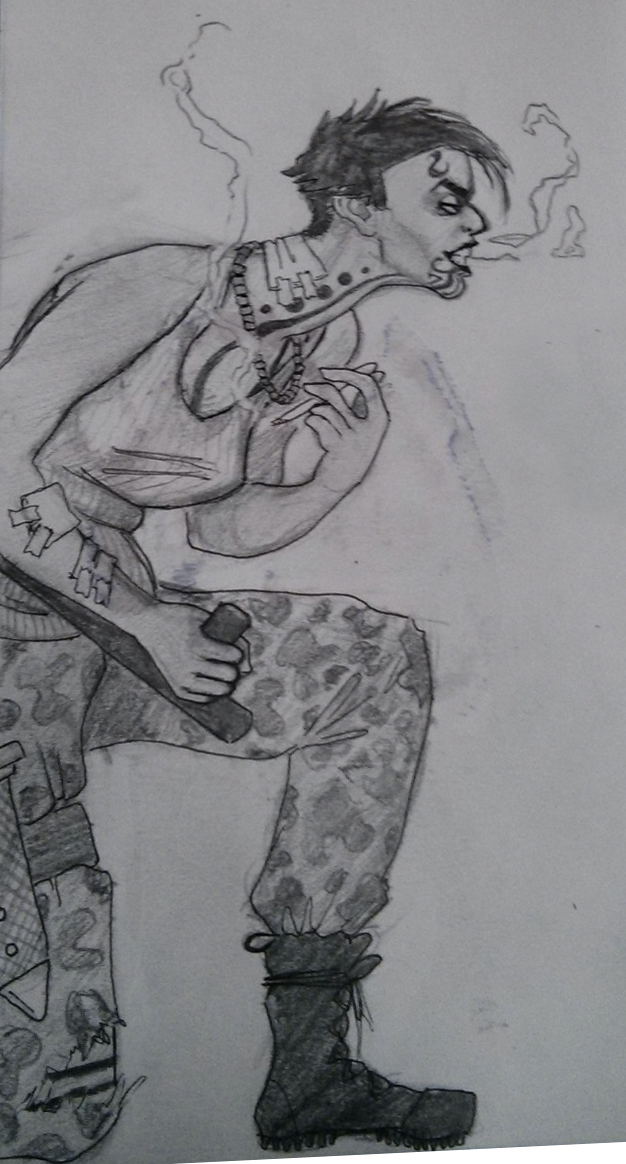
\includegraphics[width=8cm]{img/book1_jaya_thug.png}
\end{center}

\vspace{\fill}

\begin{flushright}
\textsubscript{last edited by \textbf{Nathaniel Ford} @ 05/07/15 4:28pm}
% Exported @ 08/22/15 12:58pm
\end{flushright}

